\documentclass[a4paper]{article}

%·······························································································
%                                _    _                _           
%                               | |  | |              | |          
%                               | |__| | ___  __ _  __| | ___ _ __ 
%                               |  __  |/ _ \/ _` |/ _` |/ _ \ '__|
%                               | |  | |  __/ (_| | (_| |  __/ |   
%                               |_|  |_|\___|\__,_|\__,_|\___|_|   
%·······························································································

% Packages import
\usepackage[spanish]{babel}     % Spanish language support
\usepackage[utf8]{inputenc}     % UTF-8 encoding
\usepackage[T1]{fontenc}        % Proper font encoding
\usepackage{geometry}           % Page layout
\usepackage{titlesec}           % Custom section titles
\usepackage{lmodern}            % Modern font
\usepackage{fancyhdr}           % Header and footer
\usepackage{graphicx}           % Inserting images
\usepackage{anyfontsize}        % Arbitrary font size
\usepackage{listings}           % Code formatting
\usepackage{caption}            % Caption customizing
\usepackage{float}              % Image placing
\usepackage{sourcesanspro}
\usepackage{array}
\usepackage[dvipsnames,x11names,table]{xcolor}
\usepackage[colorlinks=true,linkcolor=black,urlcolor=Emerald]{hyperref}

% Packages configurations {{{

    % Adjust margins
    \geometry{a4paper, margin=2.5cm}

    % Change font family
    \renewcommand{\familydefault}{\sfdefault}
    
    % Change default command to resize all text
    \renewcommand{\normalsize}{\fontsize{13}{16}\selectfont}

    % Change table's cells padding
    \setlength{\tabcolsep}{12pt}
    \renewcommand{\arraystretch}{1.5}
    
    % Header/Footer settings
    \fancyfoot[C]{\thepage}

    % Shell prompt code
    \lstdefinestyle{shellprompt}{
        backgroundcolor=\color{black},
        basicstyle=\fontsize{11}{20}\ttfamily\color{white},
        keywordstyle=\color{NavyBlue},
        commentstyle=\color{white},
        stringstyle=\color{green},
        breaklines=true,
    }

    % Define the style for code with line numbers
    \lstdefinestyle{normalcode}{
        numbers=left,         % Display line numbers on the left
        numberstyle=\tiny,    % Small size for the line numbers
        stepnumber=1,         % Number every line
        numbersep=5pt,        % Space between line numbers and code
        backgroundcolor=\color{lightgray}, % Background color of code block
        basicstyle=\ttfamily\footnotesize, % Set font to typewriter and small size
    }

    % Set default listings style to shellprompt
    \lstset{style=shellprompt}

% }}}

\hyphenpenalty=10000  % Avoid hyphenation
\exhyphenpenalty=10000
\sloppy  % Loosens the strictness of the justification algorithm
\newcommand{\textgap}{\vspace{1em}}

% Metadata {{{

    % Title
    \title{Sistemas Cooperativos y Gestión de Contenidos}
    
    % Author
    \author{Juan Manuel Segura Duarte}

% }}}













%·······························································································
%                     _____                                        _   
%                    |  __ \                                      | |  
%                    | |  | | ___   ___ _   _ _ __ ___   ___ _ __ | |_ 
%                    | |  | |/ _ \ / __| | | | '_ ` _ \ / _ \ '_ \| __|
%                    | |__| | (_) | (__| |_| | | | | | |  __/ | | | |_ 
%                    |_____/ \___/ \___|\__,_|_| |_| |_|\___|_| |_|\__|
%·······························································································
\begin{document}

% Cover Page
\begin{titlepage}
    \centering
    \vspace*{3cm}  % Space at the top
    {\Huge \textbf{SCGC Práctica 3}} % Custom title
    \vspace{1cm}
    
    {\Large Sistemas Cooperativos y Gestión de Contenidos: Desarrollo de la 3ª práctica} % Subtitle
    
    
\includegraphics[width=0.5\textwidth]{images/ugr-logo.png}
    \vspace{1cm}
    
    \textbf{\Large Juan Manuel Segura Duarte} % Author name
\end{titlepage}
\newpage

% Table of Contents page
\thispagestyle{empty}
\tableofcontents

%%%%%%%%%%%%%%%%%%%%%%%%%%%%%%%%%%%%%%%%%%%%%%%%%%%%%%%%%%%%%%%%%%%%%%%%%%%%%%%%%%%%%%%%%%%%%%%%%%
%%%%%%%%%%%%%%%%%%%%%%%%%%%%%%%%%%%%%%%%%%%%%%%%%%%%%%%%%%%%%%%%%%%%%%%%%%%%%%%%%%%%%%%%%%%%%%%%%%
%%%%%%%%%%%%%%%%%%%%%%%%%%%%%%%%%%%%%%%%%%%%%%%%%%%%%%%%%%%%%%%%%%%%%%%%%%%%%%%%%%%%%%%%%%%%%%%%%%

% Start numbering in this page (after the title page and index)
\newpage
\pagenumbering{arabic}
\setcounter{page}{1}

\section{Tareas realizadas}

En esta práctica se han cumplido los objetivos de configuración inicial de WordPress mediante las siguientes acciones:

\textbf{Plugins instalados y utilizados:}
\begin{itemize}
    \item Elementor: Para el diseño visual de páginas
    \item Essential Addons for Elementor: Ampliación de widgets
    \item Essential Blocks: Componentes predefinidos
    \item Gmap Block: Integración de mapas
    \item W3 Total Cache: Optimización de rendimiento
\end{itemize}

\subsection{Configuración inicial y plantilla hija}
\begin{enumerate}
    \item Instalación del tema principal \texttt{the-coffee-shop} desde el repositorio oficial
    \item Creación de plantilla hija mediante Child Theme Configurator
    \item Modificaciones básicas en el CSS para personalización de:
    \begin{itemize}
        \item Esquema de colores corporativos
        \item Tipografía principal
    \end{itemize}
    \item Configuración de zonas de widgets verificada en Apariencia $\rightarrow$ Personalizar
\end{enumerate}

\begin{figure}[H]
    \centering
    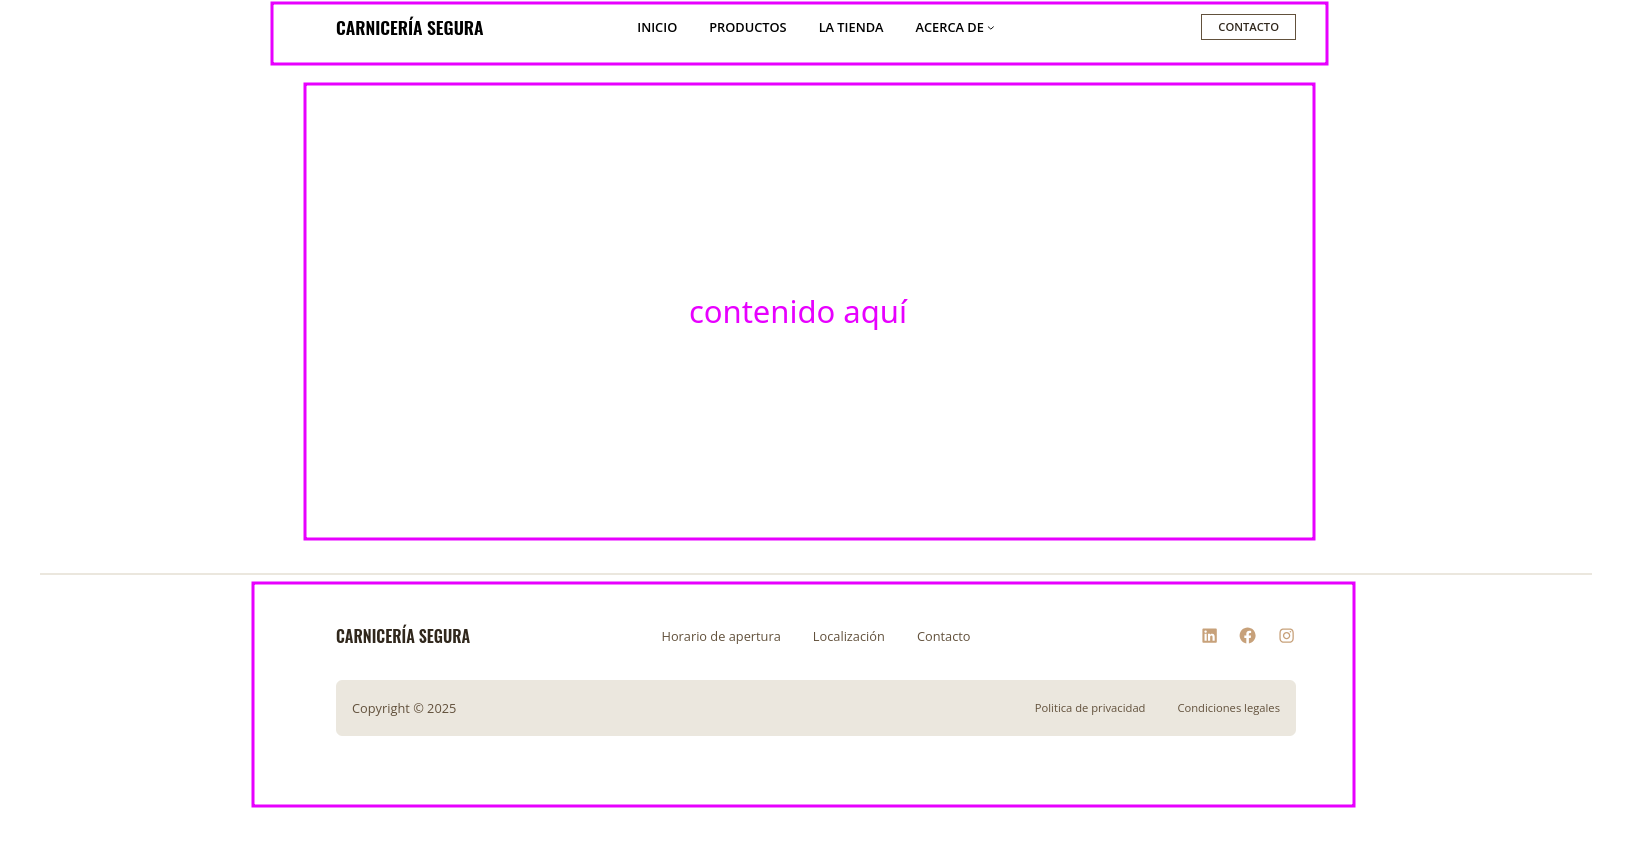
\includegraphics[width=0.85\textwidth]{images/template.png}
    \caption{Configuración inicial de la plantilla hija}
\end{figure}


\subsection{Creación de Landing Page}
\begin{enumerate}
    \item Estructura one-page con secciones scrollables
    \item Implementación con Elementor del carrusel de noticias
    \item Integración de iconos sociales en footer
    \item Optimización de carga con W3 Total Cache
\end{enumerate}

\begin{figure}[H]
    \centering
    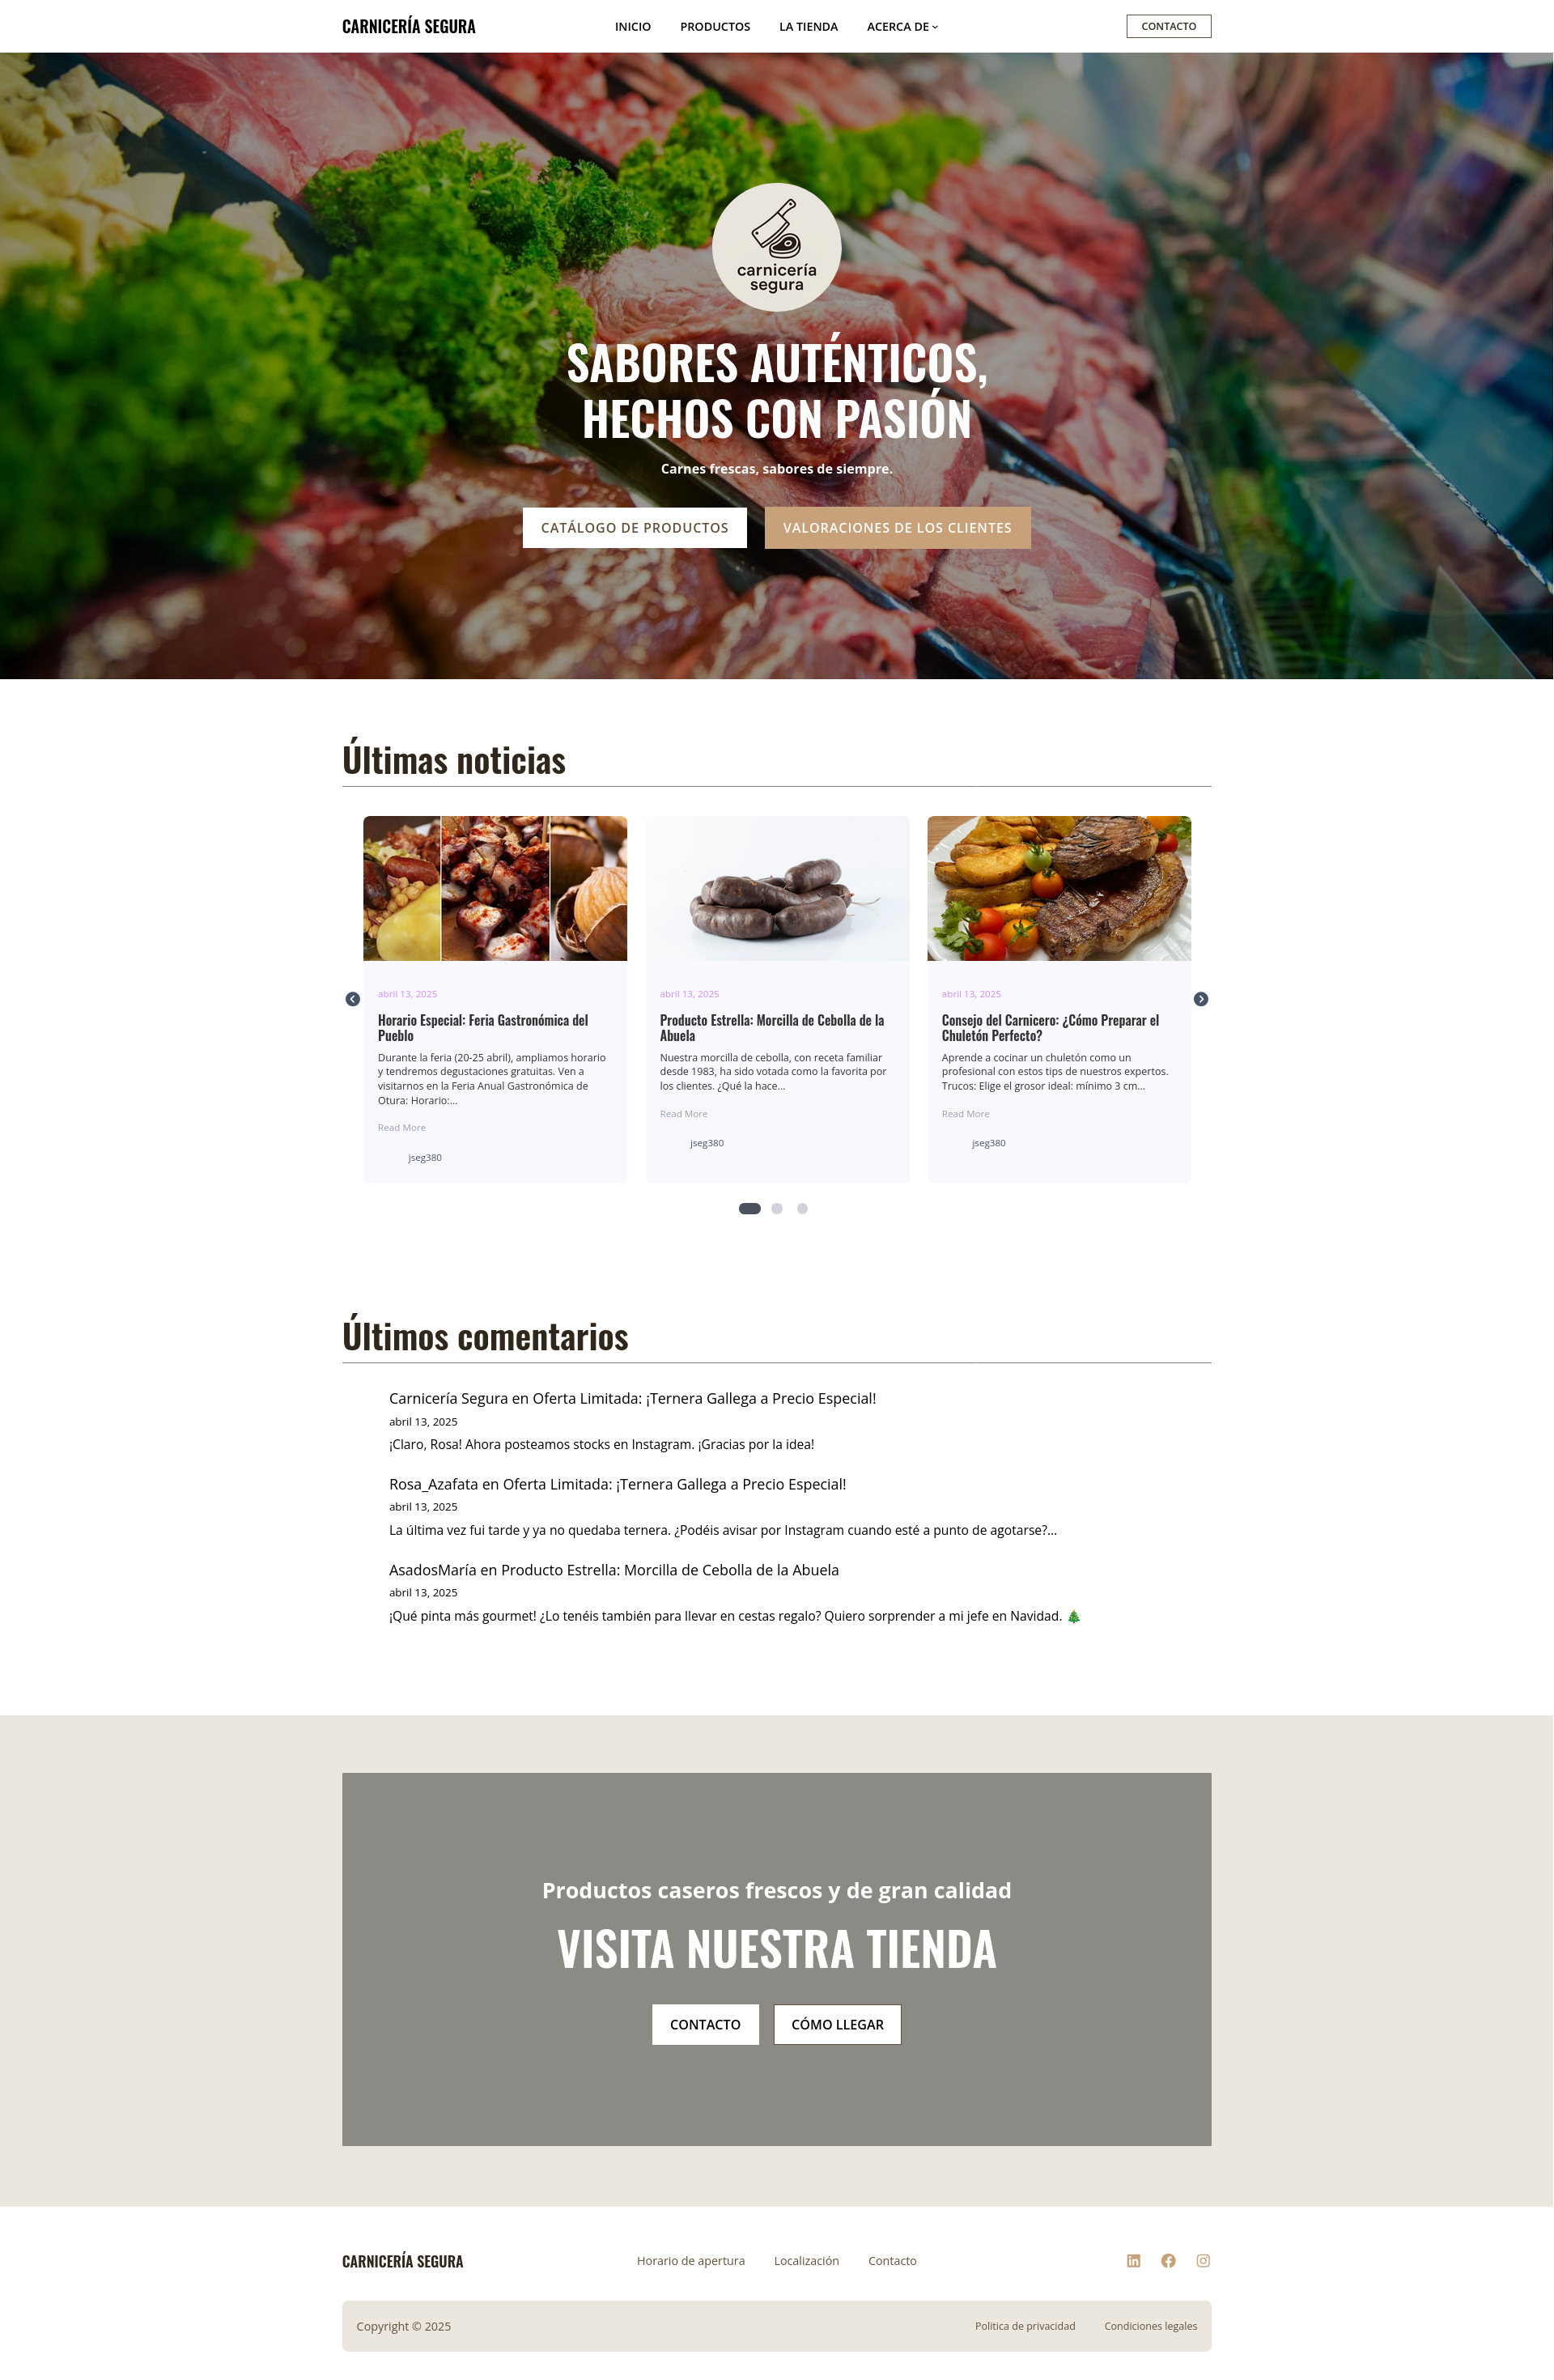
\includegraphics[width=0.85\textwidth]{images/landing-page.png}
    \caption{Interfaz de Elementor para diseño de la landing page}
\end{figure}


\subsection{Sección de noticias}
\begin{enumerate}
    \item Creación de categoría \texttt{Noticias} y 5 entradas demo
    \item Configuración de:
    \begin{itemize}
        \item Sistema de comentarios nativo
        \item Etiquetas y taxonomías básicas
        \item Widget de últimas entradas (Essential Blocks)
    \end{itemize}
    \item Vinculación desde menú principal
\end{enumerate}

\begin{figure}[H]
    \centering
    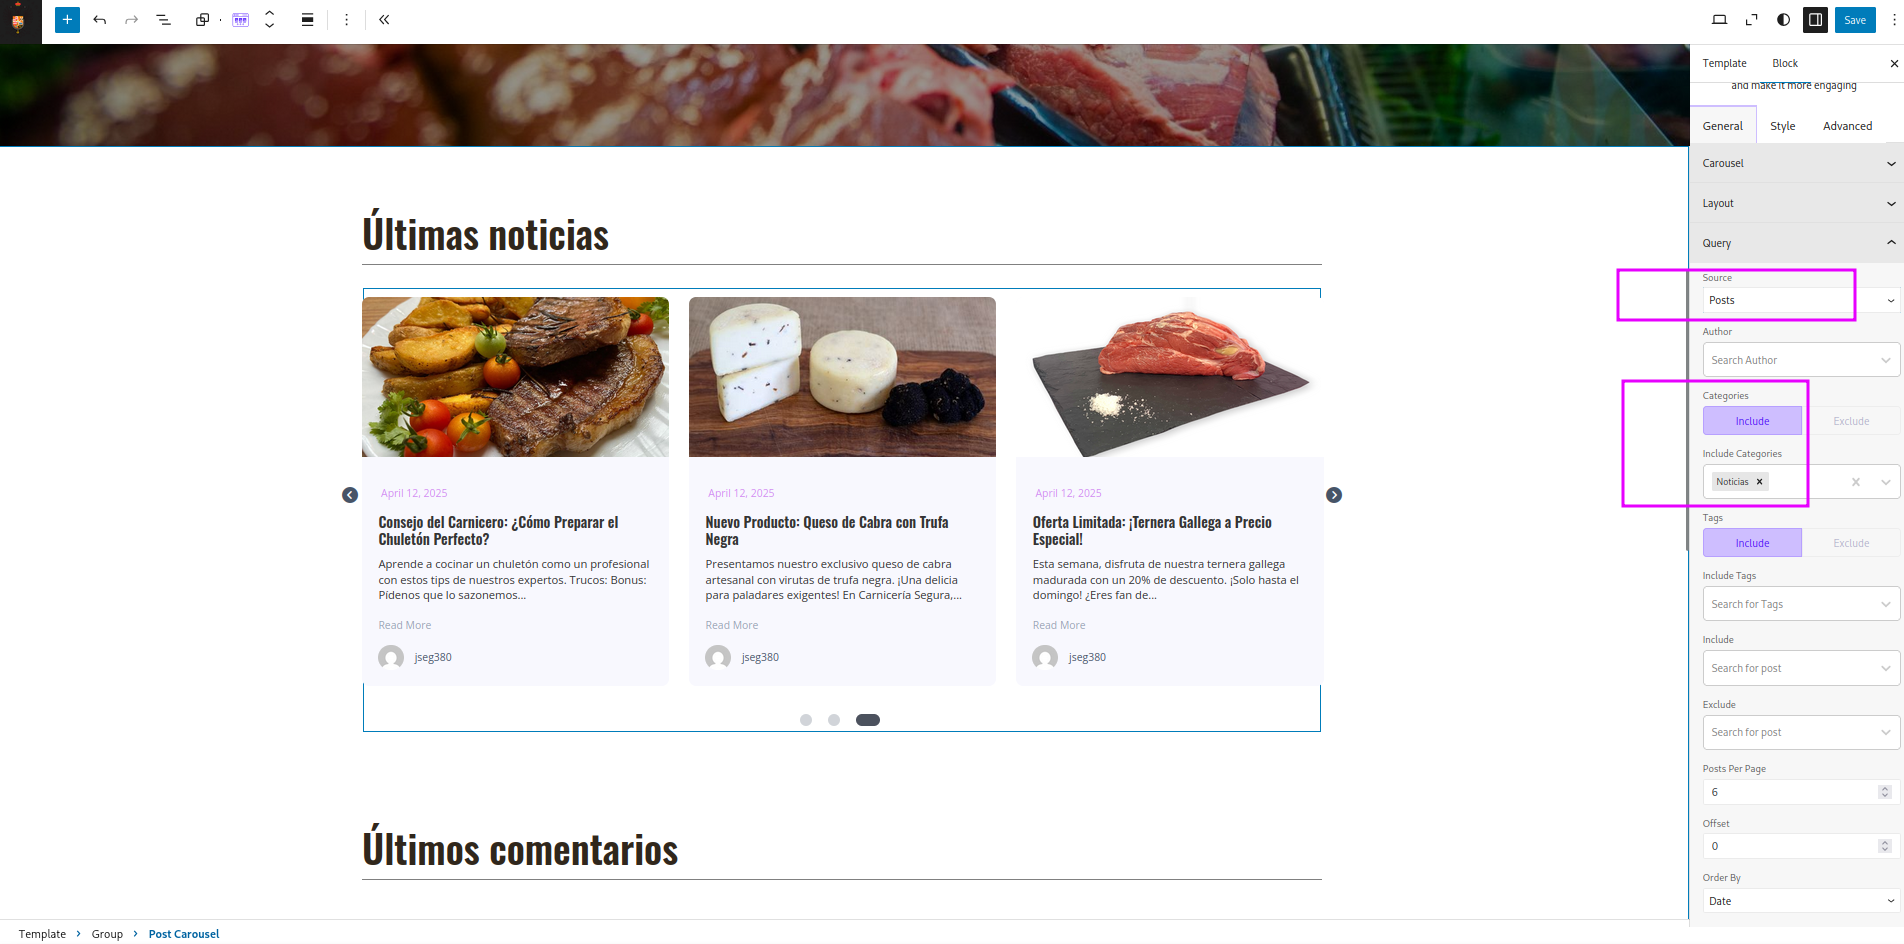
\includegraphics[width=0.85\textwidth]{images/news-section.png}
    \caption{Vista previa de la sección de noticias con widget configurado}
\end{figure}


\subsection{Páginas estáticas}
Creación de 5 páginas esenciales:

\subsubsection{Condiciones Legales}
\begin{figure}[H]
    \centering
    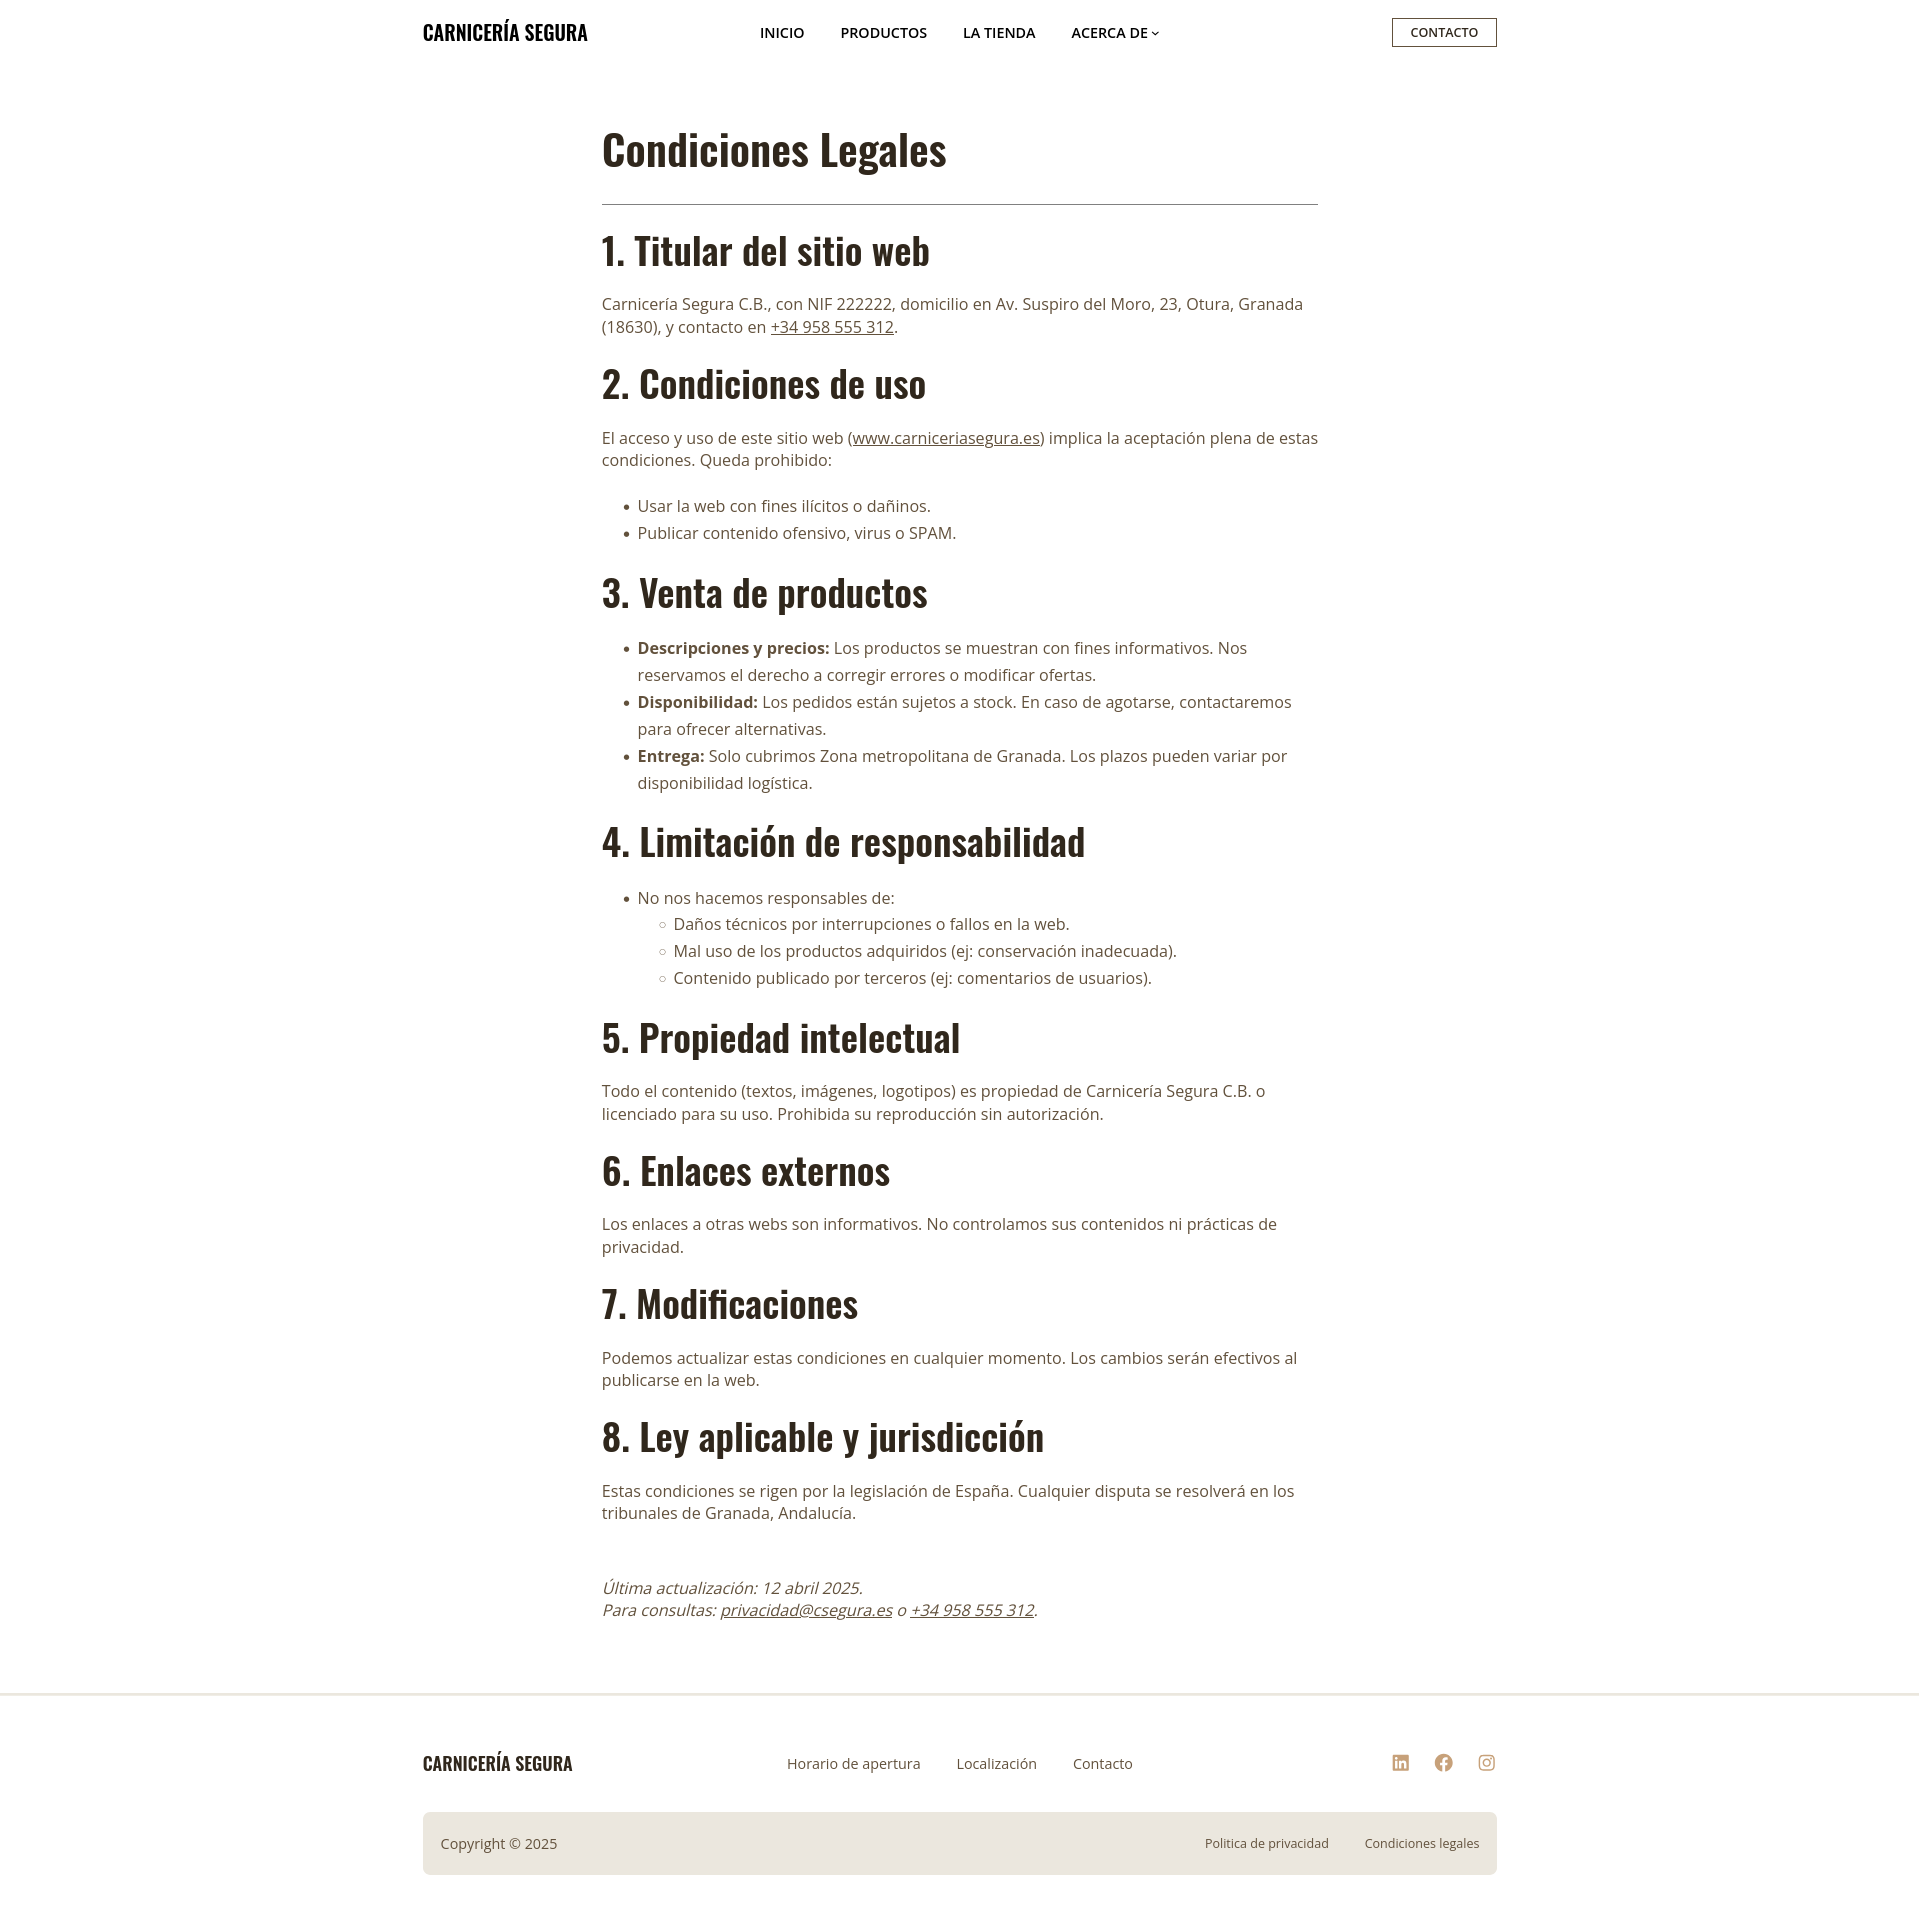
\includegraphics[width=0.85\textwidth]{images/legal.png}
\end{figure}

\subsubsection{Política de Privacidad}
\begin{figure}[H]
    \centering
    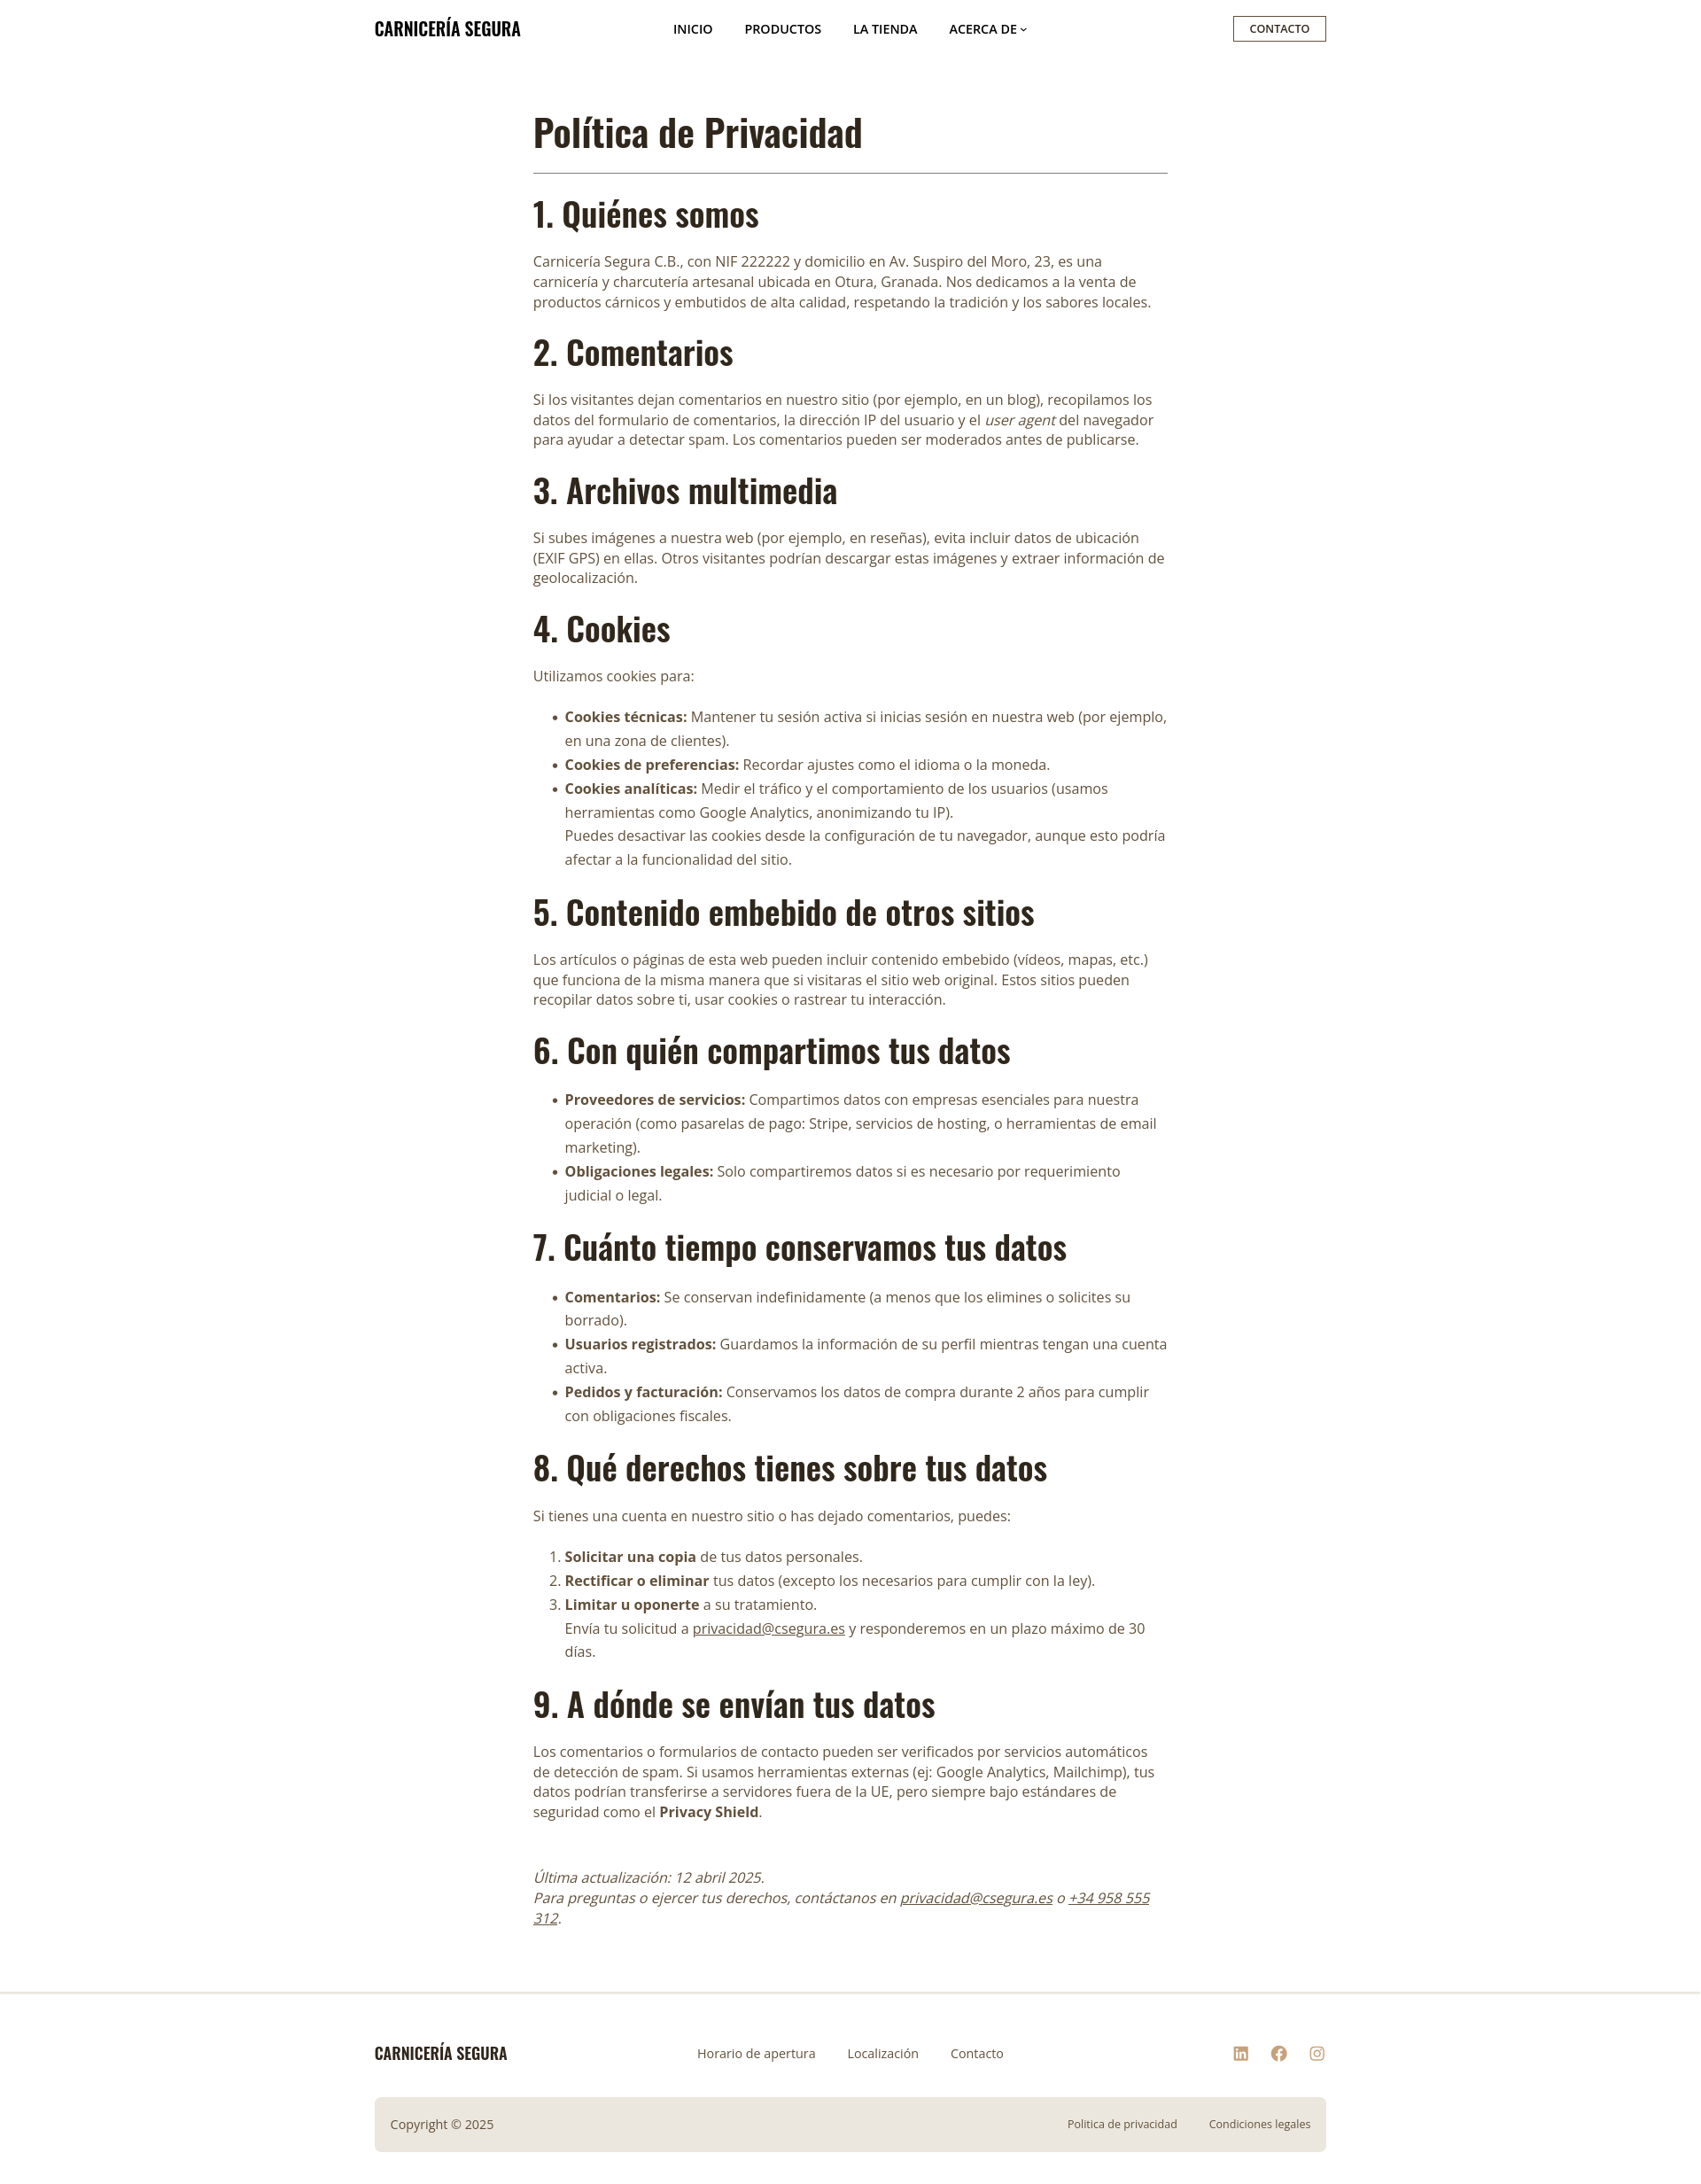
\includegraphics[width=0.85\textwidth]{images/privacy-policy.png}
\end{figure}

\subsubsection{Contacto}
\begin{figure}[H]
    \centering
    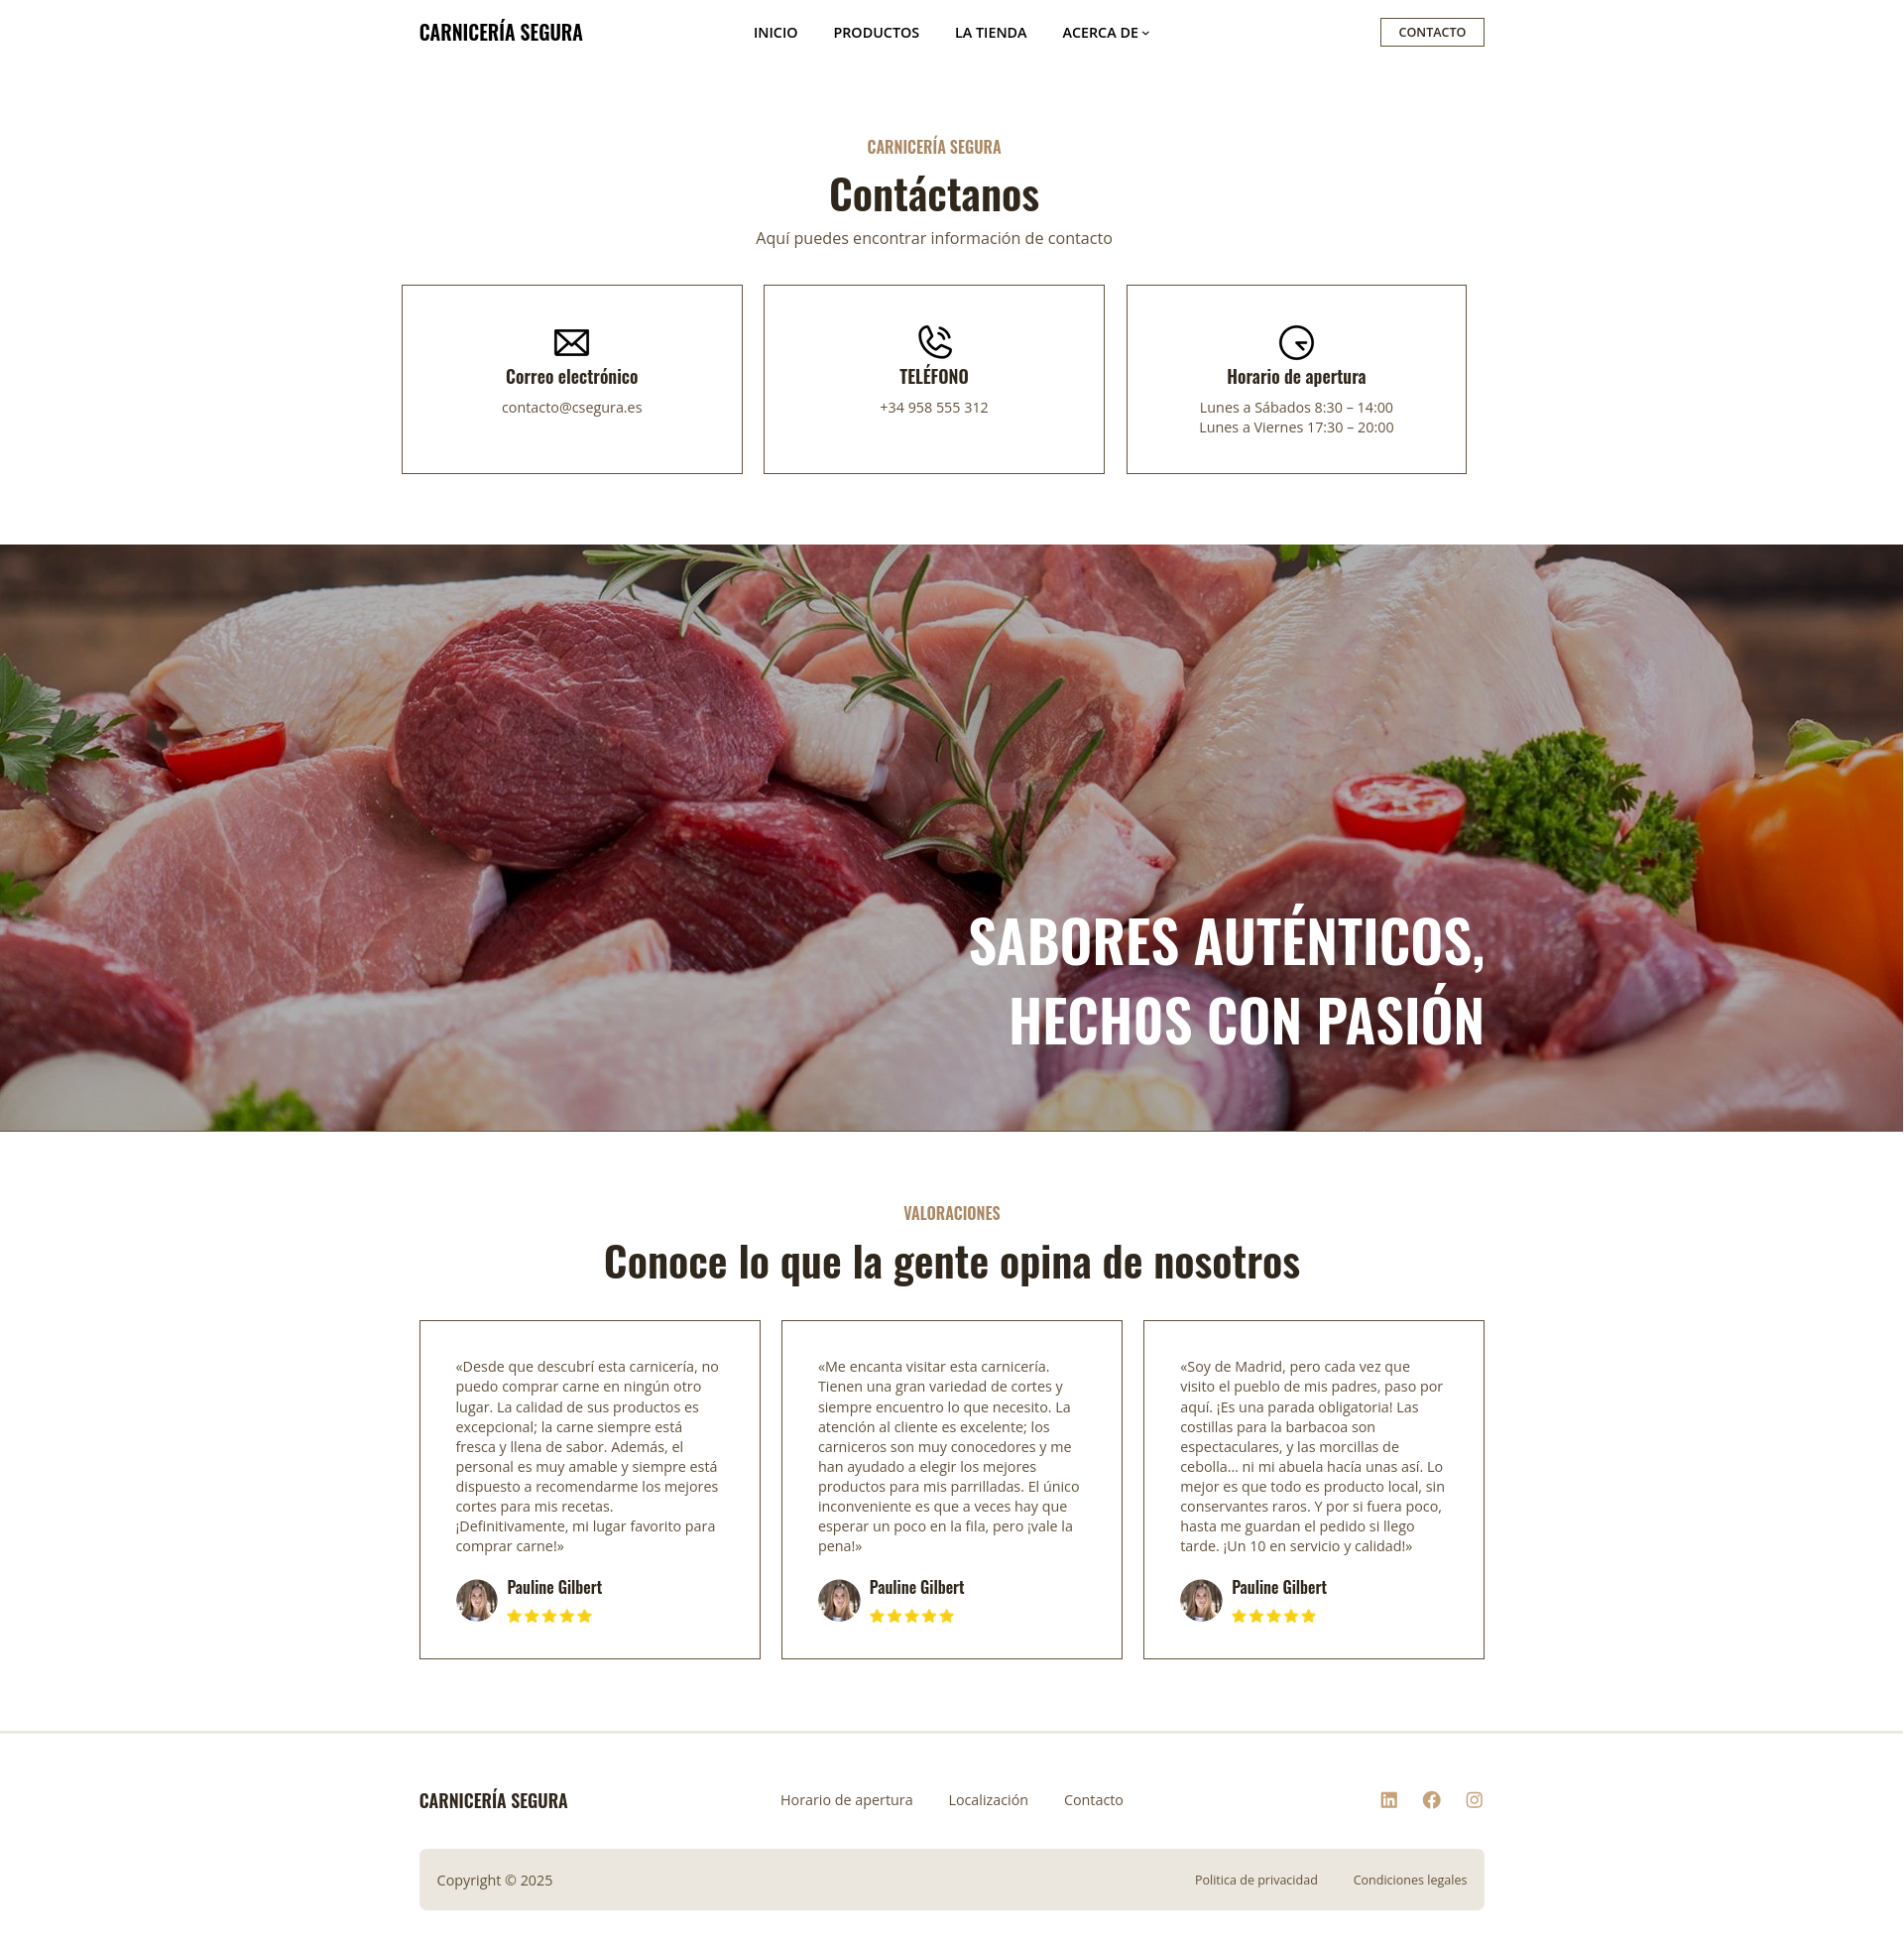
\includegraphics[width=0.85\textwidth]{images/contact.png}
\end{figure}

\subsubsection{Historia}
\begin{figure}[H]
    \centering
    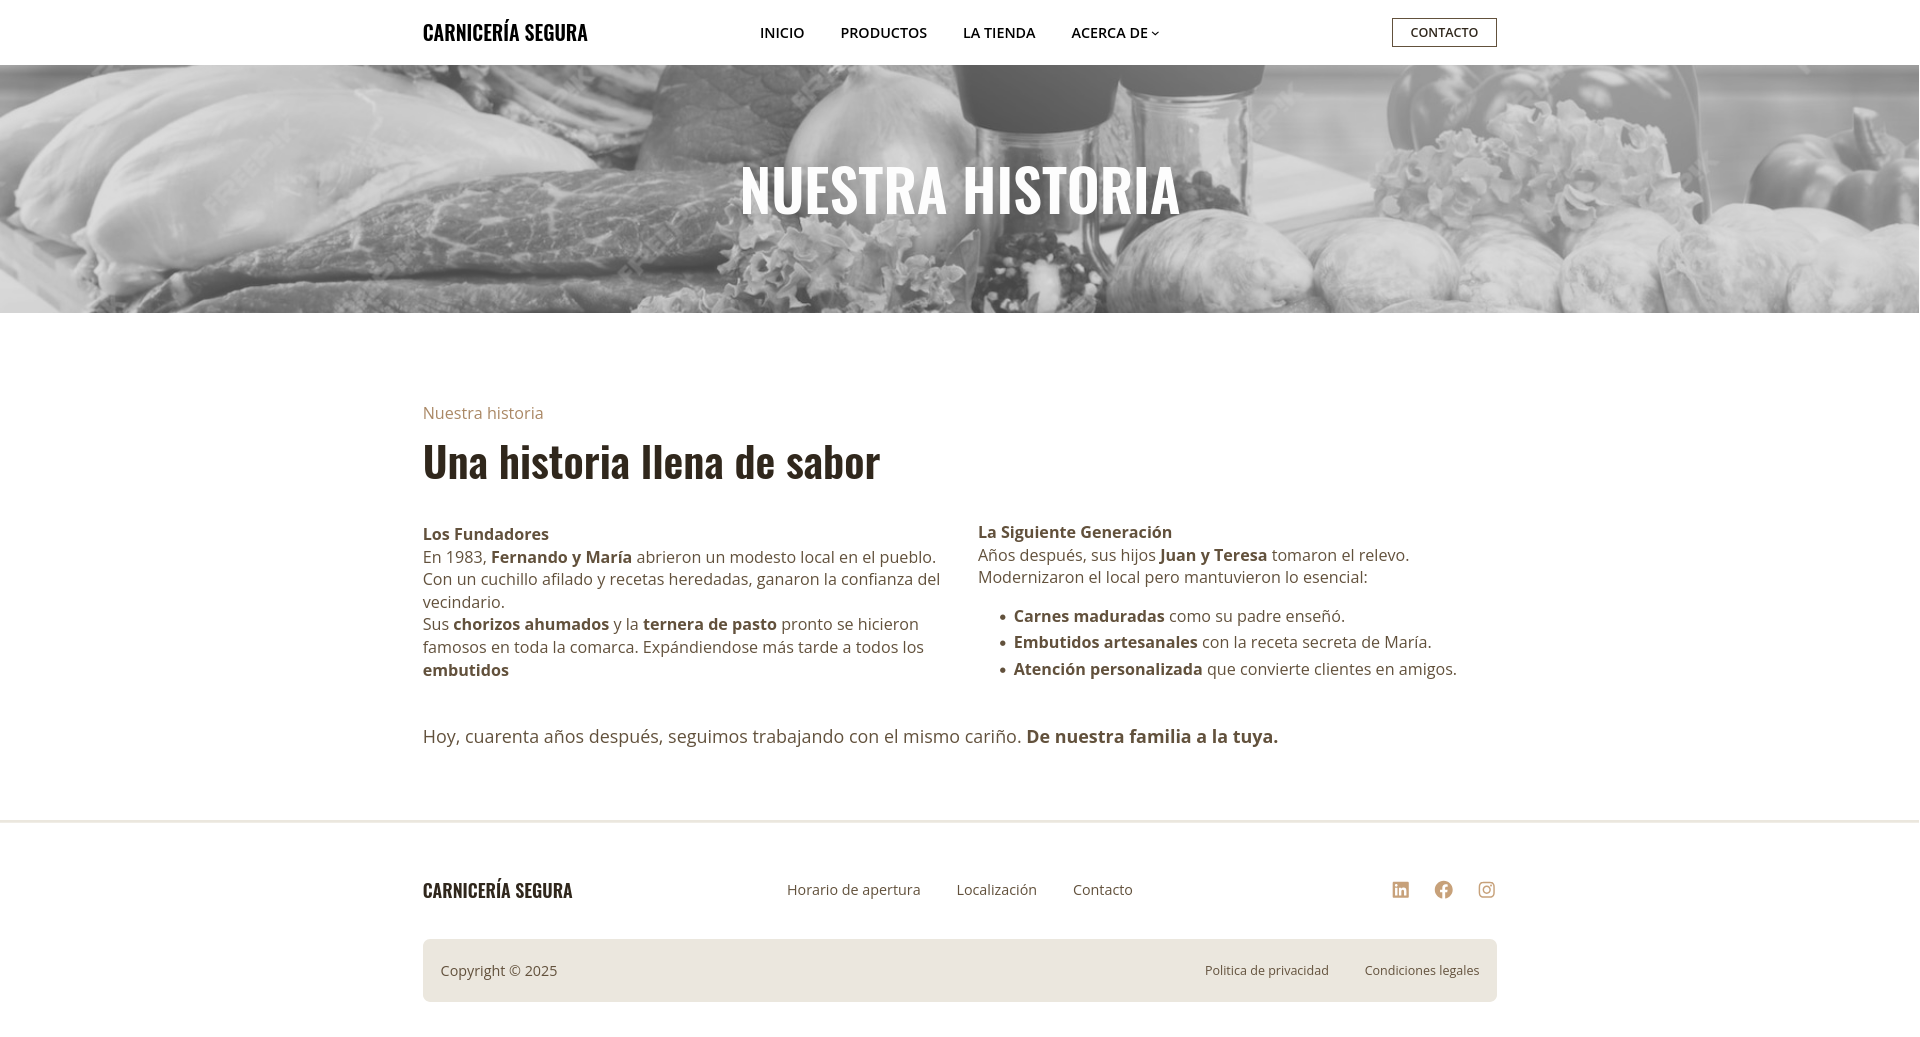
\includegraphics[width=0.85\textwidth]{images/history.png}
\end{figure}

\subsubsection{La Tienda}
\begin{figure}[H]
    \centering
    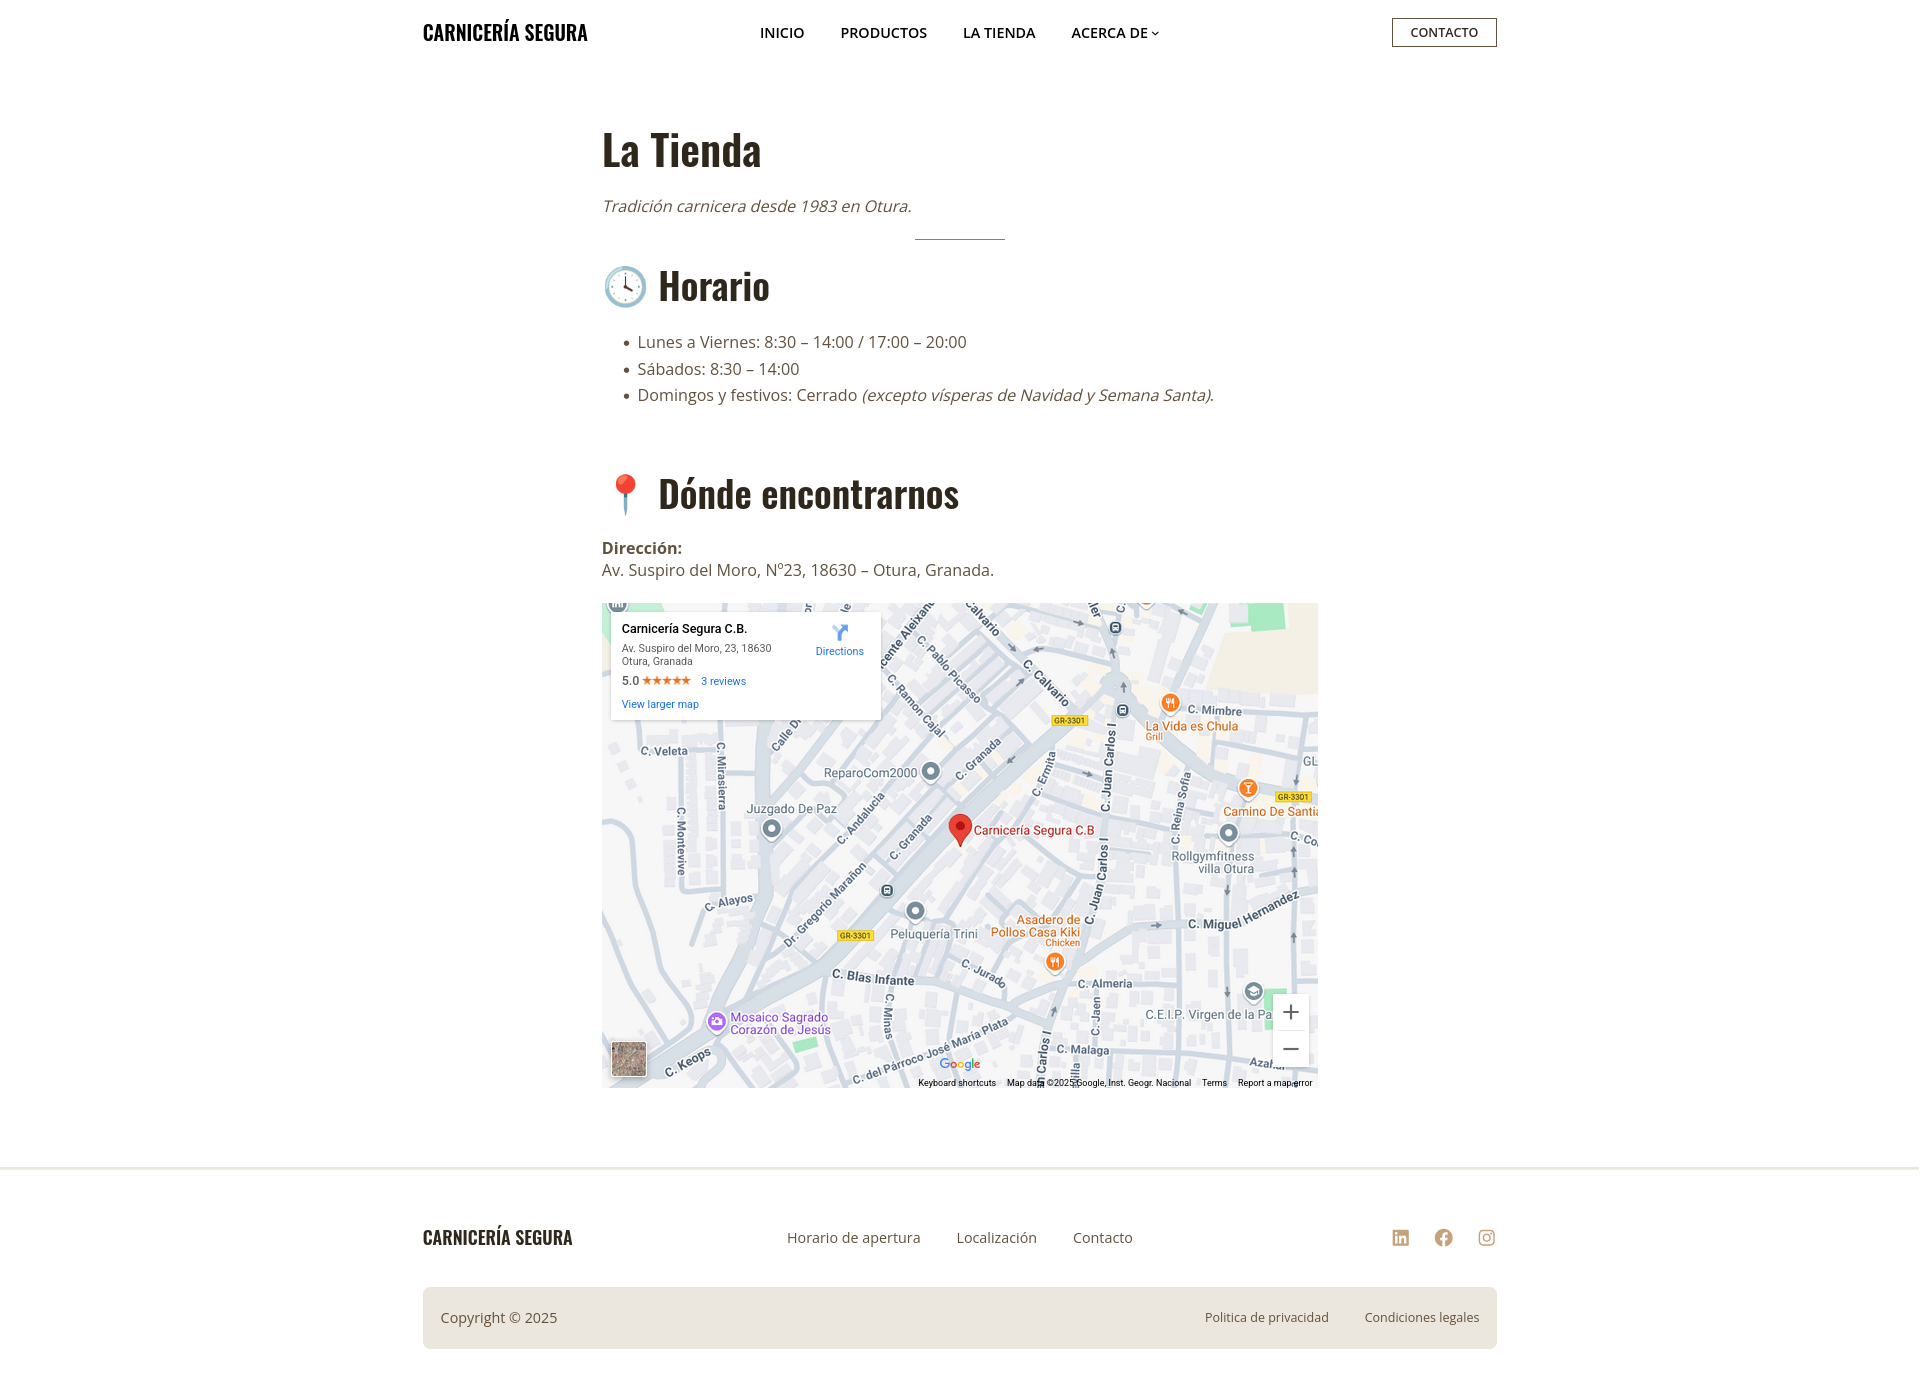
\includegraphics[width=0.85\textwidth]{images/shop.png}
\end{figure}


\section{Vídeo}

\href{https://drive.google.com/file/d/1E2T5aiZRP-RegQDz_RJMtYyBGyNKR_c_/view?usp=sharing}{Enlace al vídeo mostrando la práctica}


\end{document}
